\chapter{Campionamento: cuti, piccoli campioni e biopsie}

Il campionamento delle biopsie e delle piccole resezioni viene trattato separatamente rispetto ai campioni chirurgici, poiché questi ultimi spesso non richiedono orientamento e non necessitano di un campionamento macroscopico mirato. In altre parole, viene effettuata una selezione casuale del materiale da inviare per l'analisi, mentre il resto del materiale viene conservato per eventuali ulteriori esami. Si noti che per le resezioni di grandi dimensioni o per le radicalizzazioni post-chirurgiche può essere necessaria la conservazione del campione.

Il campionamento di solito segue procedure standardizzate, con campionamento a "caso", ovvero campionando solo una parte del materiale senza una selezione accurata. La prima sezione di questo capitolo è dedicata alle biopsie cutanee.

\section{Biopsie Cutanee}

Le biopsie cutanee possono essere eseguite in qualsiasi ambulatorio e possono essere classificate in due categorie principali: biopsie incisionali e biopsie escissionali. Le biopsie incisionali prevedono il prelievo di solo una parte della lesione, mentre le biopsie escissionali mirano all'asportazione totale del tessuto ritenuto patologico.

Tra i tipi di campioni operatori che possono essere inviati al laboratorio vi sono:

\subsection{Biopsia Punch}
La biopsia punch consiste in un prelievo a carota di tessuto, che include l'epidermide e il derma. Se il punch è eseguito in profondità, può includere anche la quota di tessuto sottocutaneo. Viene utilizzato un cilindro metallico tagliente, appoggiato sulla cute, per estrarre una carota di tessuto. I punch sono disponibili in vari diametri e vengono frequentemente utilizzati per piccole lesioni o per malattie infiammatorie della pelle. A seconda delle dimensioni del punch, si può decidere se includere l'intero campione o suddividerlo per analizzare la lesione al centro del punch stesso. In caso di malattie infiammatorie, è spesso necessario congelare metà del campione per effettuare ulteriori analisi.

\subsection{Biopsia Shave}
La biopsia shave prevede l'abrasione della lesione cutanea, che può essere piatta o rilevata, mediante l'uso di una lama. Vengono rimosse solo le porzioni più superficiali del derma. È importante indicare il margine e il piano profondo per orientare il tecnico all'inclusione e per valutare la radicalità chirurgica.


\begin{figure}[p]
    \centering
    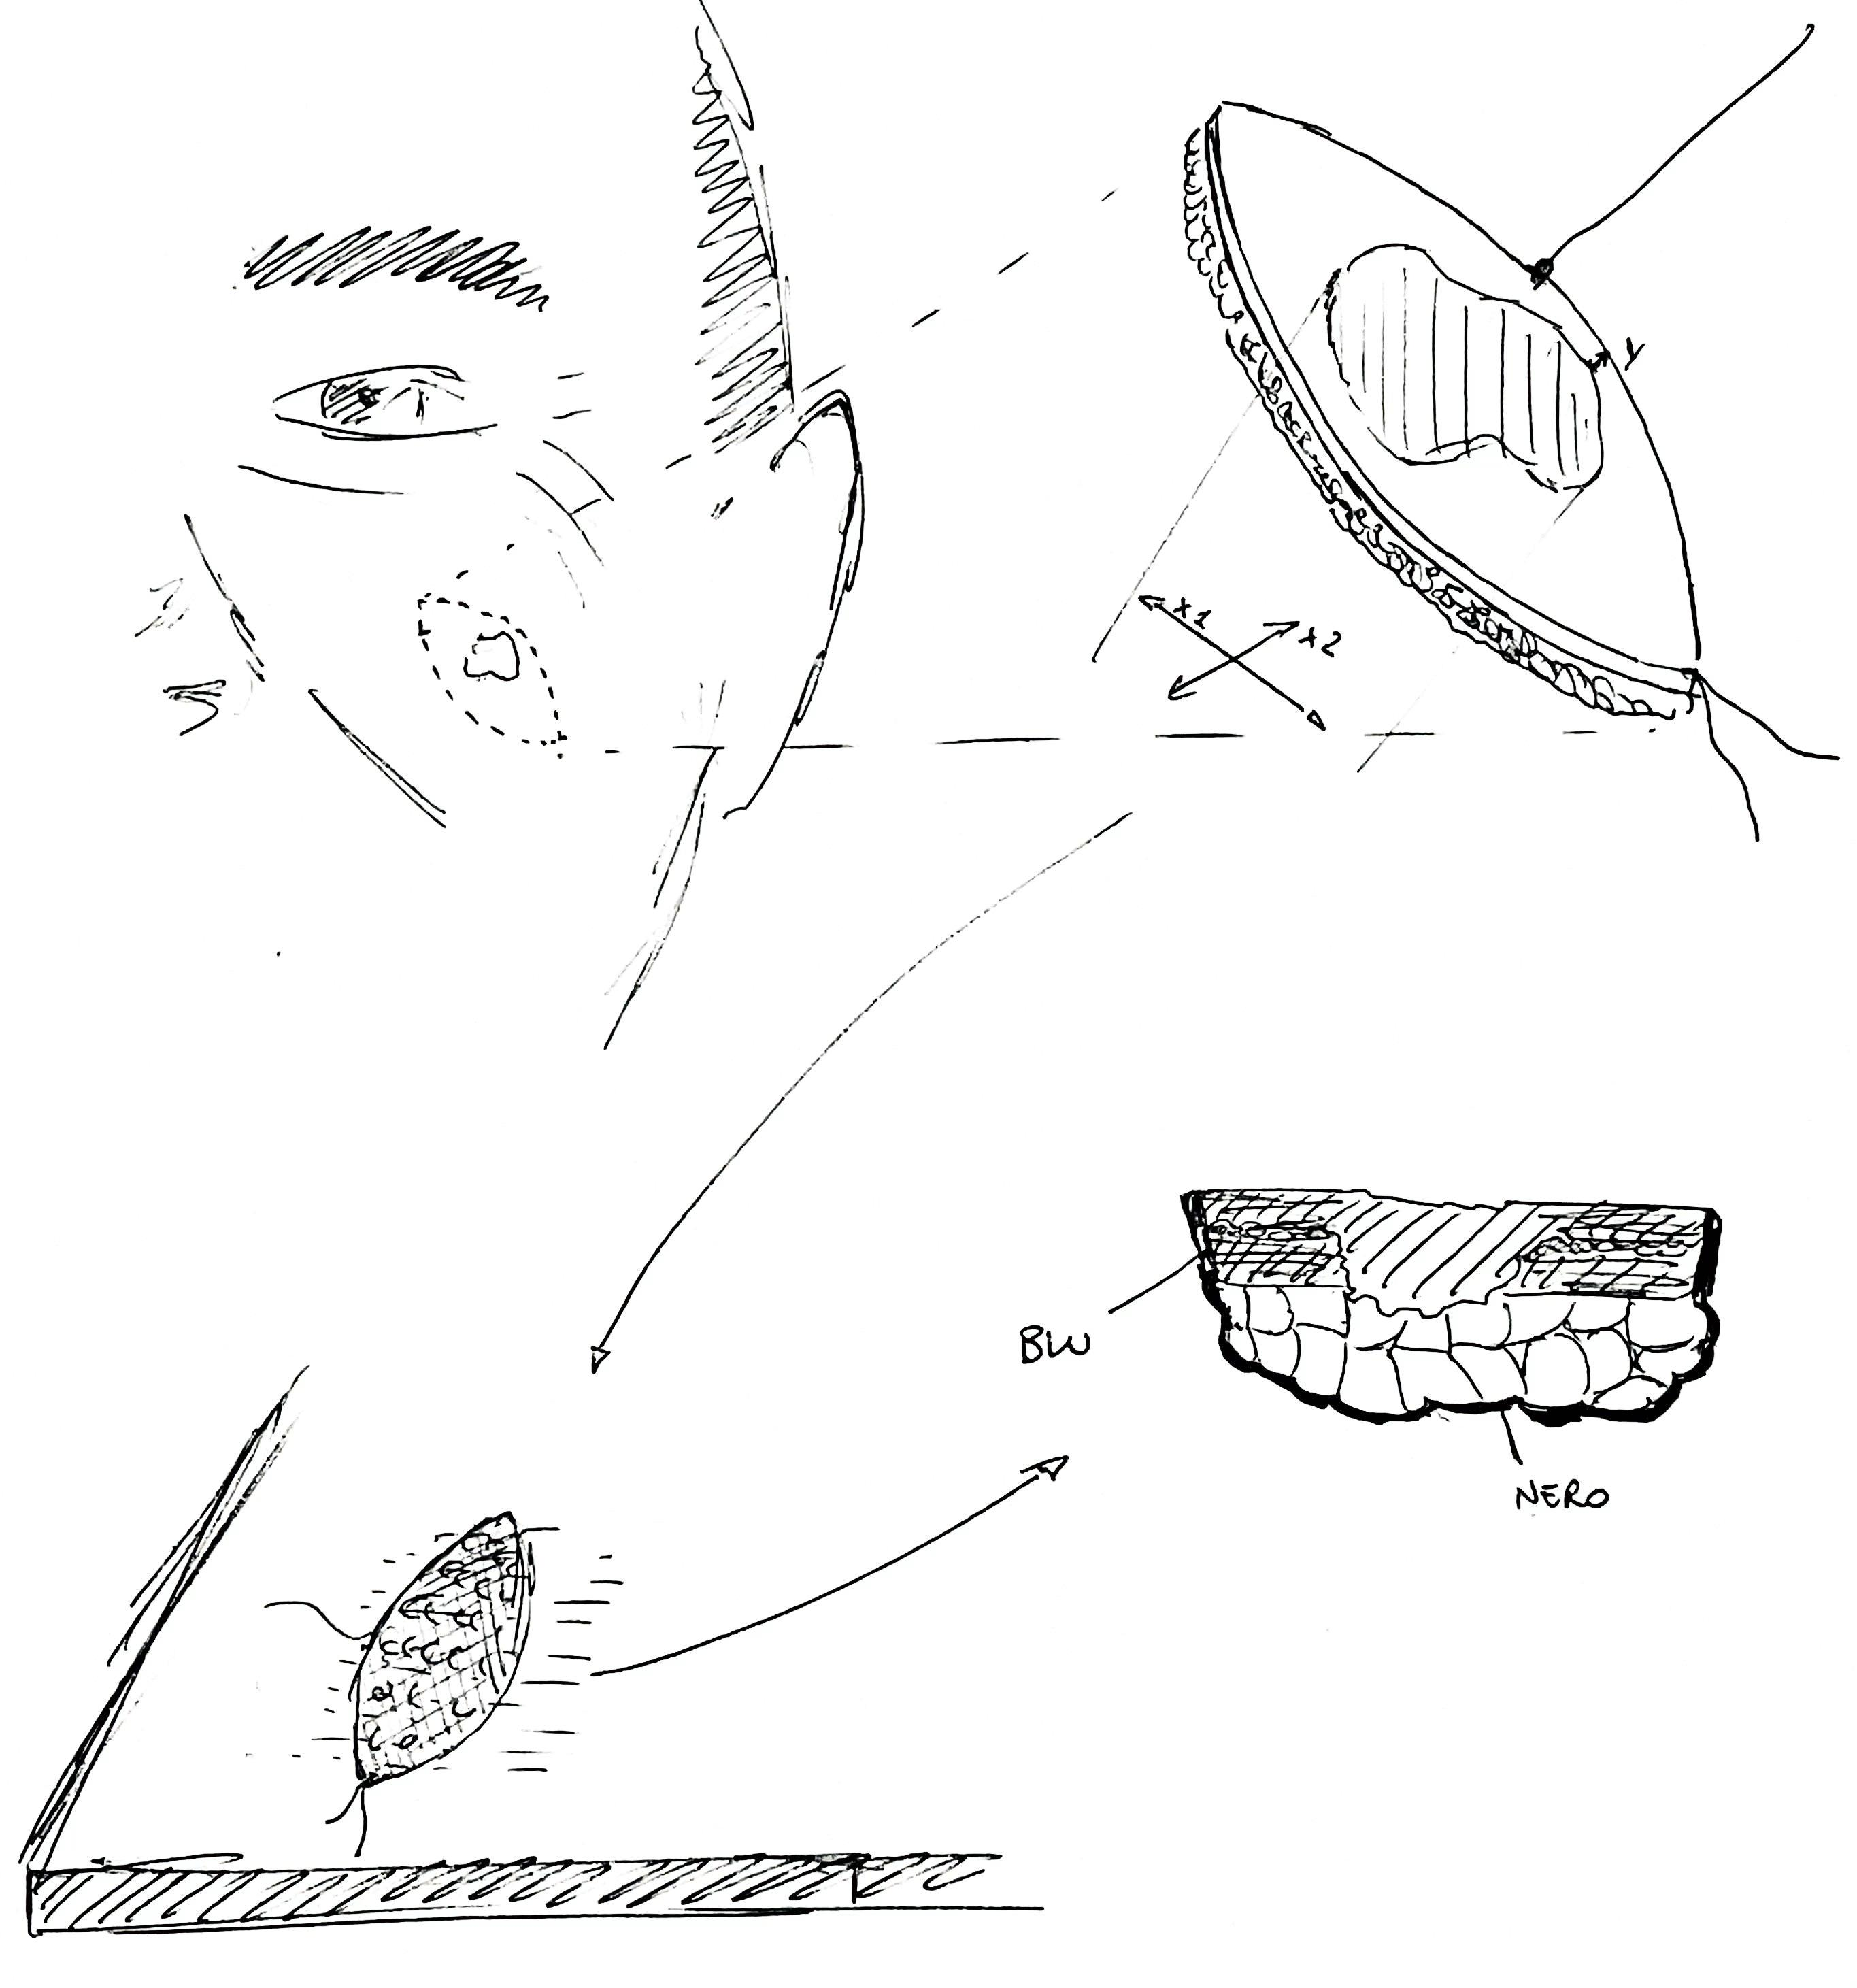
\includegraphics[width=0.75\textwidth]{campionamento_cute}
    \caption{Il campionamento delle losanghe cutanee.}
    \label{fig:campionamento_cute}
\end{figure}


\subsection{Losange Cutanee}
Le biopsie a forma di losanga prevedono un campione cutaneo con una forma romboidale, caratterizzato da due angoli acuti e due angoli arrotondati. Questa forma consente una migliore gestione chirurgica della ferita, con i due angoli acuti utilizzati come punto di partenza per la sutura. Le losange possono essere orientate, soprattutto in siti con margini ristretti, come sul volto, per facilitare l'asportazione di tessuto in caso di margine positivo.

\subsection{Descrizione Macroscopica}
Nella descrizione dei campioni cutanei è cruciale fornire dettagli macroscopici, per due motivi principali: primo, una diagnosi preliminare può essere fatta basandosi sull'aspetto macroscopico; secondo, la presenza di non concordanza tra la descrizione macroscopica e quella microscopica può suggerire ulteriori indagini. La descrizione delle neoformazioni cutanee deve includere dimensioni (in millimetri), caratteristiche morfologiche (rilevate, piatte, depressed), e dettagli sulla superficie (croste, escoriazioni, ulcere), oltre ai margini (netti o sfumati) e al colore, che è rilevante sia per lesioni melanocitarie che non melanocitarie.


\section{Campionamento delle piccole biopsie}

Il campionamento delle piccole biopsie differisce sostanzialmente da quello dei pezzi chirurgici in due aspetti fondamentali: la selezione delle aree da campionare e l'orientamento del campione. Nel caso delle piccole biopsie, spesso si procede con l'inclusione totale del materiale, senza selezionare specifiche aree come avviene nei pezzi chirurgici. Inoltre, l'orientamento non riguarda più l'identificazione anatomica dei margini, bensì la necessità di mostrare chiaramente le relazioni tra i diversi strati tissutali o la disposizione dei frustoli all'interno del bocchetto.

\subsection{Biopsie endoscopiche}

Le biopsie endoscopiche possono variare da piccoli frammenti difficilmente orientabili a resezioni più ampie e complesse, talvolta orientate. Un esempio significativo sono le resezioni endoscopiche sottomucose, in cui il campionamento deve permettere di osservare chiaramente tutti gli strati del tessuto, dalla mucosa alla sottomucosa. Questi campioni richiedono una particolare attenzione nella preparazione e nell'inclusione, per garantire che le sezioni seriate mostrino tutte le strutture rilevanti sul vetrino.

\subsection{Campionamento delle Biopsie Endoscopiche}
Le biopsie endoscopiche possono variare da semplici frammenti a resezioni di grandi dimensioni. Questi campioni spesso arrivano in formalina e sono difficilmente orientabili. Tuttavia, quando si tratta di resezioni sottomucose (resezione della mucosa separata dalla muscolare tramite endoscopia), l'orientamento è cruciale. 
\textbf{Punti principali per il campionamento}:
\begin{itemize}
    \item Rimozione del pezzo dal supporto con delicatezza dopo fissazione.
    \item Sezionamento seriate delle resezioni e inclusione orientata in modo che tutti gli strati, dalla mucosa alla sottomucosa, siano visibili sul vetrino.
    \item I margini apicali vanno campionati separatamente.
\end{itemize}


\subsection{Resezioni Endoscopiche Orientate}
Le resezioni endoscopiche orientate, come quelle fissate su supporti con spilli, devono essere trattate in modo specifico. La parte importante è campionare in maniera tale che le sezioni seriate includano la rappresentazione completa degli strati del campione.
\\ \textbf{Punti di attenzione}:
\begin{itemize}
    \item Orientamento a 90° rispetto alla posizione originaria del campione.
    \item Inclusione delle sezioni in modo da vedere chiaramente tutti gli strati tessutali.
\end{itemize}

\subsection{Resezioni Transuretrali Prostatiche (TURP)}
Le resezioni transuretrali prostatiche richiedono un campionamento che segue criteri specifici:
\begin{itemize} 
    \item Pesatura del materiale per determinare il numero di cassette necessarie.
    \item Campionamento minimo di cinque cassette per resezione (indicativamente 15 g).
    \item Un'ulteriore cassetta ogni 10 g di materiale resecato.
   \item in caso di diagnosi di carcinoma all'istologia il materiale viene successivamente incluso in toto.
\end{itemize}
L'obiettivo è garantire che non vi siano tumori prostatici nascosti, pur trattando resezioni per patologie non oncologiche come l'ipertrofia prostatica.

\subsection{Frustoli da core needle biopsy}

I cilindri di tessuto ottenuti tramite core biopsy rappresentano un'altra sfida per il campionamento. A causa della loro forma e della tendenza a piegarsi durante la fissazione, è importante cercare di mantenere il tessuto il più lineare possibile. Questo può essere ottenuto utilizzando spugnette o carta per mantenere i frustoli dritti e allineati, facilitando una corretta inclusione e minimizzando la perdita di tessuto durante la lavorazione. Inoltre, nel caso di campioni più ampi o multipli, può essere utile distribuire i frustoli su più cassette, soprattutto se si prevede la necessità di ulteriori sezioni o esami molecolari.

Le \textit{core biopsies}, ovvero biopsie a cilindro, devono essere trattate in modo da ottimizzare la fissazione e inclusione. 
\\ \textbf{Aspetti pratici per le core biopsies}:
\begin{itemize}
    \item Utilizzo di spugnette per mantenere i frustoli diritti durante la fissazione.
    \item Stendere i frustoli in modo che non si pieghino, per evitare che si perda parte della superficie utile.
    \item Dividere su più cassette nel caso di campioni abbondanti o quando si prevede di eseguire ulteriori analisi (coronazioni o esami molecolari).
\end{itemize}

\subsection{Biopsie Framementate e Biopsie Core}
Per le biopsie frammentate, si raccomanda di campionare abbondantemente in caso di sospetto diagnostico. In caso di dubbio, si dovrebbe consultare un patologo esperto per decidere come procedere. 

\section{Riassunto}

Il campionamento delle piccole biopsie differisce dal campionamento dei pezzi chirurgici per la mancanza di un criterio specifico di selezione delle aree e per un diverso approccio all'orientamento.  Le biopsie cutanee possono essere incisionali o escissionali. Tra le tecniche, vi sono la biopsia punch, che preleva un cilindro di tessuto cutaneo, la biopsia shave, che rimuove solo le porzioni superficiali del derma, e le losanghe cutanee, usate per una gestione ottimale della ferita. La descrizione macroscopica di questi campioni è essenziale per una diagnosi accurata. Le biopsie endoscopiche richiedono un'attenzione particolare nella preparazione per assicurare che tutte le strutture rilevanti siano visibili, mentre le resezioni transuretrali prostatiche (TURP) seguono un campionamento basato sul peso. Nel caso delle core biopsy, è importante mantenere i frustoli allineati per facilitare l'inclusione e ottimizzare la quantità di tessuto a disposizione per la diagnosi.

